%% LaTeX-Beamer template for KIT design
%% by Erik Burger, Christian Hammer
%% title picture by Klaus Krogmann
%%
%% version 2.1
%%
%% mostly compatible to KIT corporate design v2.0
%% http://intranet.kit.edu/gestaltungsrichtlinien.php
%%
%% Problems, bugs and comments to
%% burger@kit.edu

\documentclass{beamer}

%% SLIDE FORMAT

% use 'beamerthemekit' for standard 4:3 ratio
% for widescreen slides (16:9), use 'beamerthemekitwide'

\usepackage{templates/beamerthemekitwide}
% \usepackage{templates/beamerthemekitwide}

\usepackage[utf8]{inputenc}
\usepackage[T1]{fontenc}
\usepackage{lmodern}
\usepackage[ngerman]{babel}
\usepackage{amsmath}
\usepackage{amssymb}
\usepackage{graphicx}
\usepackage{booktabs}
\usepackage{mathabx}
\usepackage{eurosym}
\usepackage{nameref}

%% TITLE PICTURE

% if a custom picture is to be used on the title page, copy it into the 'logos'
% directory, in the line below, replace 'mypicture' with the
% filename (without extension) and uncomment the following line
% (picture proportions: 63 : 20 for standard, 169 : 40 for wide
% *.eps format if you use latex+dvips+ps2pdf,
% *.jpg/*.png/*.pdf if you use pdflatex)

%\titleimage{mypicture}

%% TITLE LOGO

% for a custom logo on the front page, copy your file into the 'logos'
% directory, insert the filename in the line below and uncomment it

%\titlelogo{mylogo}

% (*.eps format if you use latex+dvips+ps2pdf,
% *.jpg/*.png/*.pdf if you use pdflatex)

%% TikZ INTEGRATION

% use these packages for PCM symbols and UML classes
\usepackage{templates/tikzkit}
\usepackage{templates/tikzuml}

\graphicspath{{logos/}, {./images/}}


% the presentation starts here

\title{GIT}
\subtitle{Eine Einführung}
\author[Dominic]{Dominic Heun}
\institute{AES Ettlingen - TGJ2/2}
\date{\today}

% \institute{Chair for Software Design and Quality

\AtBeginSection[]
{
  \begin{frame}
    \begin{center}
    \tableofcontents[currentsection]
    \end{center}
  \end{frame}
}

\begin{document}

  % change the following line to "ngerman" for German style date and logos
  % \selectlanguage{ngerman}

  \setbeamercovered{invisible} % make next text in beamer invisible

  %title page
  \begin{frame}[plain]
    \titlepage
  \end{frame}

  \section{Was ist GIT}

  \begin{frame}{Wie arbeitet man im Team mit eigenen Computern}
    \begin{itemize}[<+->]
      \item Synchronisation?
      \item[$\Rightarrow$] Fehleranfällig oder mehrere arbeiten gleichzeitig?
      \item[$\Rightarrow$] GIT löst Problem
    \end{itemize}
  \end{frame}

  \begin{frame}{Versionskontrolle}
      \begin{columns}
        \column{0.6\textwidth}

          \begin{itemize}[<+->]
            \item Verschiedene Versionen
            \item Jeder arbeitet an seinen \textit{Versionen} der Dateien
            \item \textbf{Commit} gibt die Information weiter
            \item \textbf{Merge} fügt die verschiedenen Versionen zusammen
          \end{itemize}

        \column{0.4\textwidth}
          \begin{figure}
            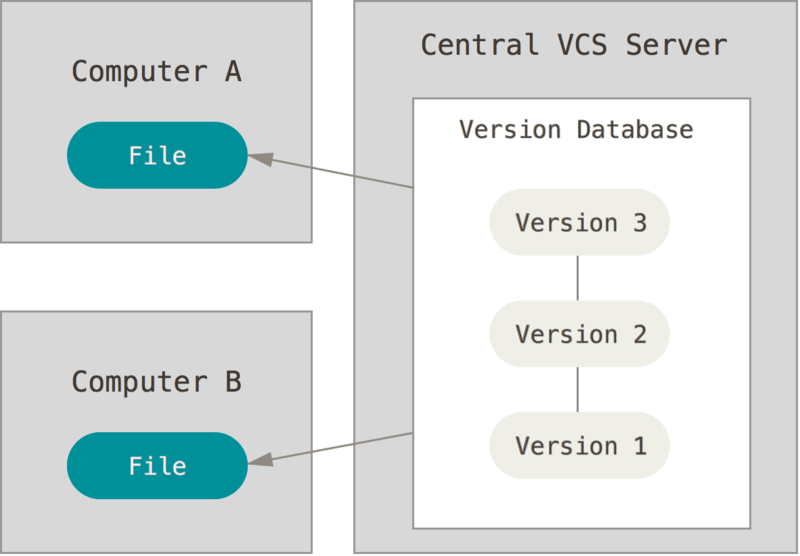
\includegraphics[width=0.9\columnwidth]{version-control-centralized}
            \caption{
              Versionskontrolle mit zentralem VCS Sever
              \tiny{
                \url{git-scm.com/book/en/v2/images/centralized.png}; 08.05.2018
              }
            }
          \end{figure}
      \end{columns}
  \end{frame}

  \section{Git als VCS}

    \begin{frame}{Git}
      \begin{columns}
        \column{0.7\textwidth}
          \begin{itemize}[<+->]
            \item Eine Möglichkeit unter vielen (\textit{SVN, Git, Mercurial...})
            \item Entwickelt von Linus Torwalds für den \textbf{Linux Kernel}
          \end{itemize}
        \column{0.3\textwidth}
          
\includegraphics[width=0.9\columnwidth]{git}
      \end{columns}
    \end{frame}

  \section[Einrichtung]{Einrichten einer Repository}

    \begin{frame}{Clone}
      \framesubtitle{Eine Repository aus dem Internet laden}
      \begin{itemize}
        \item Repository laden
        \item Verschiedene Anbieter Möglich \begin{itemize}
                                              \item GitLab
                                              \item GitHub
                                              \item Bitbucket
                                            \end{itemize}
      \end{itemize}
      \onslide<+>{
        \begin{block}{Command}
          \texttt{git clone <url>}
        \end{block}
      }
      \onslide<+>{
        \begin{block}{Eine Repository Clonen}
          \url{https://github.com/TheDome/githubPresentation2019.git}
        \end{block}
      }
    \end{frame}

    \begin{frame}{Init}
      \begin{itemize}
        \item Repository erstellen
      \end{itemize}
      \begin{block}{Command}
        \texttt{git init}
      \end{block}
    \end{frame}

    \section[Ändern]{Änderungen Speichern}

    \begin{frame}{Add}
      \begin{itemize}[<+->]
        \item Dateien \textit{Stagen}
        \item[$\rightarrow$] Auf commit vorbereiten
        \item Mehrere Dateien nacheinander für einen Commit vorbereiten
      \end{itemize}
      \begin{block}{Command}
        \texttt{git add files..}
      \end{block}
    \end{frame}

    \begin{frame}{Commit}
      \begin{itemize}
        \item Hinzufügen von Änderungen
        \item Lädt Änderung direkt in den GIT Baum
      \end{itemize}
      \begin{block}{Command}
        \texttt{git commit -m "<Message"> files..}
      \end{block}
    \end{frame}

    \begin{frame}{Remove}
      \begin{itemize}
        \item Dateien mit GIT löschen
        \item<+-> Eigentlich auch durch löschen und commit möglich
        \item<.-> Zeichnet direkt in dem Versionsbaum auf
        \item<+-|@alert> [-r] Nimmt hierbei \textbf{alle} Dateien in einem Verzeichnis
      \end{itemize}
      \begin{block}{Command}
        \texttt{git rm [-r] [--] "<file">...}
      \end{block}
    \end{frame}

    \begin{frame}{Differences}
      \begin{columns}
        \column{0.6\textwidth}
          \begin{itemize}[<+->]
            \item Änderungen gar nicht mehr bewusst
            \item Durchsuchen
            \item Wissen, wann Änderung gemacht wurde
          \end{itemize}
          \begin{block}{Command}
            \texttt{git diff "<file">}
          \end{block}

        \column{0.4\textwidth}
          \begin{block}{Output eines diff}

          \end{block}
      \end{columns}
    \end{frame}

  \section[Merge]{Zusammenführen der Arbeit}


    \begin{frame}{Branches}
      \begin{itemize}
        \item<+-> \textit{Zweige}
        \item<+-> Möglichkeit, verschiedene \textbf{Versionen} zu haben
      \end{itemize}
      \begin{columns}
        \onslide<+->{
            \column{0.5\textwidth}
              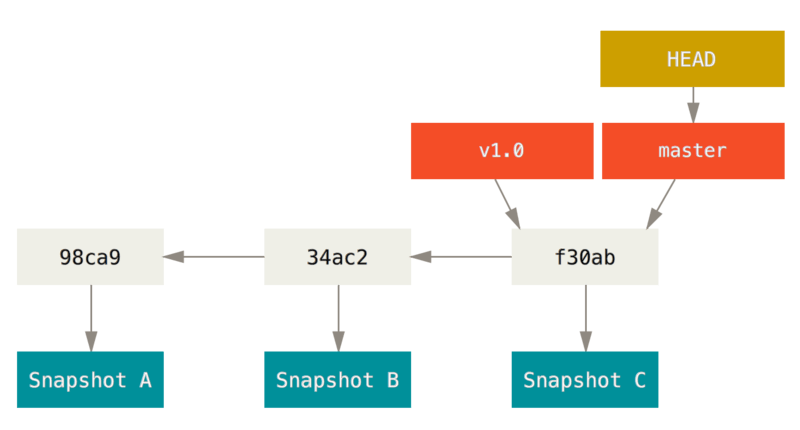
\includegraphics[width=0.9\columnwidth]{before-branch}
        }
        \onslide<+->{
            \column{0.5\textwidth}
              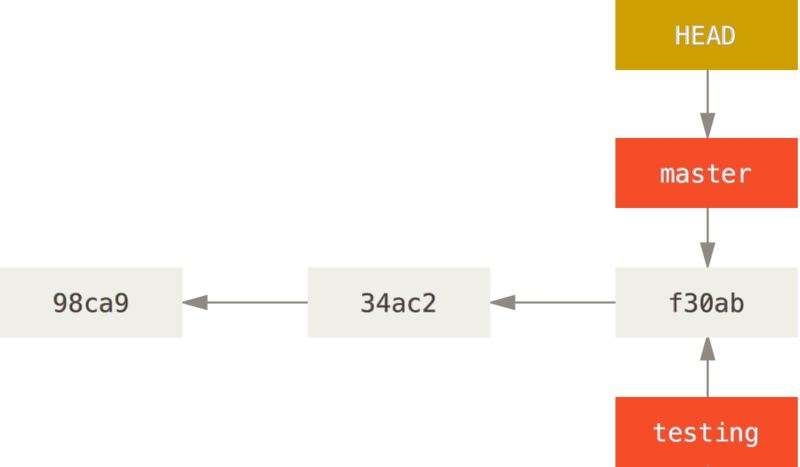
\includegraphics[width=0.9\columnwidth]{create-branch}
        }
       \end{columns}
      \tiny{Bilder von \url{git-scm.com/book/en/v2/Git-Branching-Branches-in-a-Nutshell}}
    \end{frame}

    \begin{frame}{Branches anzeigen}
      \begin{itemize}
        \item<+-> Anzeigen aller Branches
      \end{itemize}
      \onslide<+->{
        \begin{block}{Command}
          \texttt{git branch}
        \end{block}
      }
      \onslide<+->{
        \begin{block}{Ausgabe}
          \texttt{\$ git branch \\ % Show all branches later
              \onslide<+->{ iss53 \\
                * master \\
                  testing
              }
          }
        \end{block}
      }
    \end{frame}

    \begin{frame}{Branches Zusammenführen}
      \begin{columns}
        \column{0.5\textwidth}
          \begin{itemize}[<+->]
            \item Verschiedene Versionen
            \item[$\rightarrow$] Man will auf eine Version
          \end{itemize}

        \column{0.5\textwidth}
          \onslide<.->{
            \begin{figure}
              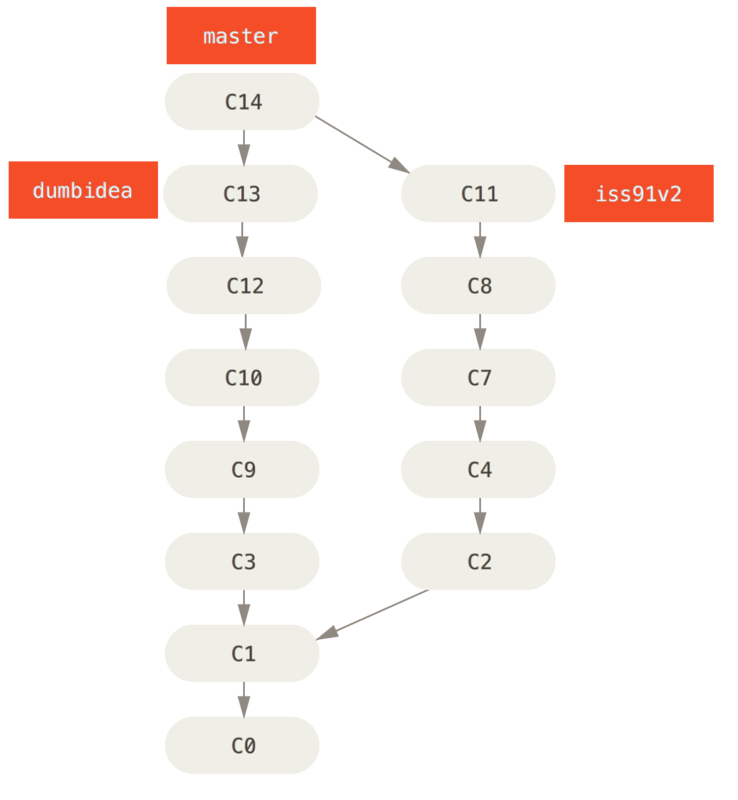
\includegraphics[height=0.68\textheight,keepaspectratio=true]{branch-different}
              \caption{Verschiedene Branches \tiny{\url{git-scm.com/book/en/v2/Git-Branching-Branching-Workflows}, 08.05.2019}}
            \end{figure}
          }
      \end{columns}
    \end{frame}

    \begin{frame}{Merge}
      \begin{columns}
        \column{0.6\textwidth}
          \begin{itemize}[<+->]
            \item Branches Zusammenführen
            \item Manche haben Konflikte
            \item[$\Rightarrow$] Selbst lösen
          \end{itemize}
          \onslide<+->{
            \begin{block}{Command}
              \texttt{git merge [<commit>...]}
            \end{block}
          }
        \column{0.4\textwidth}
          \onslide<1->{
            \begin{figure}
              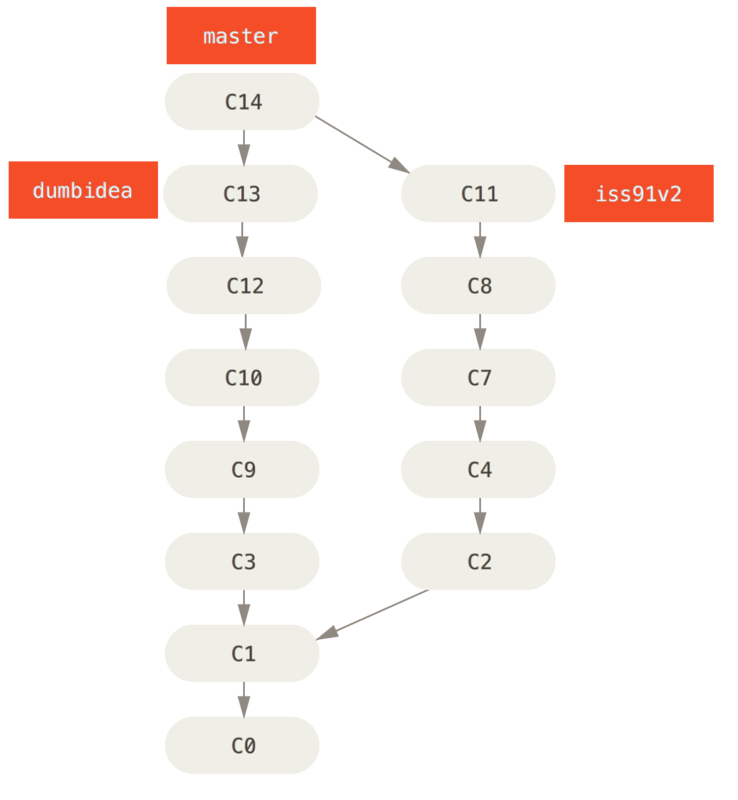
\includegraphics[height=0.68\textheight,keepaspectratio=true]{branch-different}
              \caption{Verschiedene Branches \tiny\url{git-scm.com/book/en/v2/Git-Branching-Branching-Workflows}, 08.05.2019}
            \end{figure}
          }
      \end{columns}
    \end{frame}

  \section[Status]{Den Status der Repository anzeigen}

  \begin{frame}{Status}
        \begin{itemize}[<+->]
          \item Keinen überblick über Dateien, die schon committed sind
          \item git weiß es
        \end{itemize}
        \onslide<+->{
          \begin{block}{Command}
            \texttt{git status}
          \end{block}
        }
  \end{frame}

  \begin{frame}{Log - Die Historie}
        \begin{itemize}[<+->]
          \item Keinen überblick über Dateien, die schon committed sind
          \item git weiß es
        \end{itemize}
        \onslide<+->{
          \begin{block}{Command}
            \texttt{git status}
          \end{block}
        }
  \end{frame}


\end{document}
